\DiaryEntry{Minimum Spanning Trees - Kruskal Algorithm}{2020-03-24}{Algorithms}

We consider weighted graphs $G$; i.e. each edge is assigned a weight according to some weight function $w(u,v)$, where $u,v$ are graph vertices. A spanning tree $T$ is an acyclic graph (i.e. a tree) $T \subseteq G$ which connects all vertices. A minimum spanning tree is a spanning tree whose total weight

\bee
w(T) = \sum_{(u,v) \in T} w(u,v)
\eee

is minimized (over all spanning trees).

\paragraph{Example.} To understand the problem better, we consider the following example graph.

\begin{figure}[H]
\centering
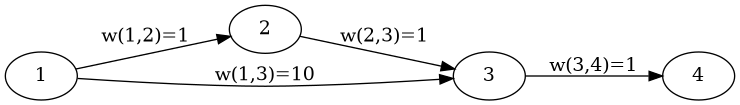
\includegraphics[scale=0.4]{images/mst_1_1.png}
\end{figure}

The graph has a cycle ($1-2-3$) and the weight of the edge $(1,3)$ is much higher than the other weights (which are all the same). Executing the Kruskal algorithm (which creates a minimum spanning tree) yields the following result. We see that the expensive edge $(1,3)$ got removed, otherwise no changes were made.

\begin{figure}[H]
\centering
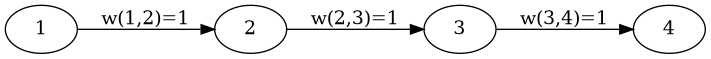
\includegraphics[scale=0.4]{images/mst_1_2.png}
\end{figure}


\subsection{Generic Algorithm}

A minimum spanning tree is generated by means of a greedy algorithm. The algorithm manages a set of edges $\Ac$ and grows it by adding one ``suitable'' edge per iteration. The algorithm maintains the following loop invariant: Prio to each iteration, the set $\Ac$ is a subset of some mininum spanning tree. At each step, the algorithm chooses an edge $(u,v)$ that can be added to $\Ac$ such that the loop invariant is fulfilled. Such an edge is called a \emph{safe} edge; it is safe in the sense that it maintains the loop invariant.

We can write down this algorithm as follows.

\begin{Verbatim}[numbers=left, xleftmargin=5mm]
Generic-MST(G, w)
   A = 0
   while A does not form a spanning tree
      find an edge (u,v) that is safe for A
      A = A + (u,v)
   return A
\end{Verbatim}

The loop invariant is kept as follows: In line 2, the empty set is a subset of a minimum spanning tree. Since we add only safe edges (lines 4, 5), we keep a subset of an MST. 

The tricky part of the algorithm is to find safe edges (line 4) in a graph. There are two ways to achieve this; one of them results in Kruskal's algorithm, the other in Prim's algorithm.

There is a rule how we can find safe edges in a graph which we will describe next. First, some definitions are required: A \emph{cut} $(S,V-S)$ of a Graph $G = (V,E)$ is a partition of the vertex set $V$ into $S$ and $V-S$. An edge $(u,v)$ \emph{crosses} the cut $(S,V-S)$ if one of its endpoints is in $S$ and the other is in $V-S$. A cut \emph{respects} a set of edges if no edge in the set crosses the cut. An edge is a \emph{light egde} crossing the cut if its weight is the minimum of any edge crossing the cut (there can be more than one light edge, if there is a tie in the weights).

A safe edge can be found as follows.

\begin{theorem}
Let $G = (V,E)$ be a connected, undirected graph with a real-valued weight function $w$ defined on $E$. Let $A$ be an edge subset that is included in some in some MST for $G$, let $(S,V-S)$ be a cut of $G$ that respects $A$, and let $(u,v)$ be a light edge crossing the cut $(S,V-S)$.Then, the edge $(u,v)$ is a safe edge for $A$.
\end{theorem}

The following Figure shows an illustrationof the above theorem. Black vertices belong to $S$, white vertices to $V-S$. The edge $(c,d)$ is the light edge as (i) it crosses the cut, and (ii) has mininum weight over all crossing edges; these are $(a,h), (b,h), (b,c), (c,d), (d,f), (e,f)$. 

\begin{figure}[H]
\centering
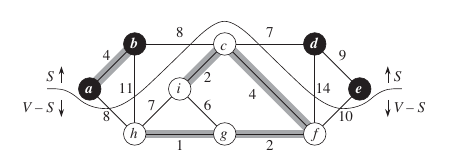
\includegraphics[scale=0.7]{images/mst_1_3.png}
\end{figure}


\subsection{Kruksal's Algorithm}

Kruskal’s algorithm finds a safe edge to add to the growing forest by finding, of all the edges that connect any two trees in the forest, an edge $(u,v)$ of least weight. Let $C_1$ and $C_2$ denote the two trees that are connected by $(u,v)$. Since $(u,v)$ must be a light edge connecting $C_1$ to some other tree, the previous theorem implies that $(u,v)$ is a safe edge for $C_1$. Kruskal’s algorithm qualifies as a greedy algorithm because at each step it adds to the forest an edge of least possible weight.

The implementation below uses a disjoint-set structure to maintain several disjoint sets of vertices (each being part of a tree). One set containing vertex $v$ is created via \verb make-set(v) . Each set has a unique ID, and there is a procedure \verb find-set(u) which takes a vertex and returns the ID of the set the vertex is in. We can use this to determine if two vertices $u, v$ are in the same tree by comparing the results of \verb find-set(u) and \verb find-set(v) . Two trees (i.e. two disjoint sets, one containing vertex $u$, the other containing vertex $v$) can be joined via \verb union(u,v) .

Then the Kruksal algorithm looks as follows

\begin{Verbatim}[numbers=left, xleftmargin=5mm]
MST-Kruksal(G, w)
   A = 0
   for each vertex v in G.V
      make-set(v)
   sort the edges of G.E into non-decreasing order by weight w
   for each edge (u,v) of G.E taken in non-decreasing order by weight
      if find-set(u) != find-set(v)
         A = A + (u,v)
         union(u,v)
   return A
\end{Verbatim}


Lines 2 - 4 initialize the result set $A$. The for loop in lines 6 - 9 run through all edges in order of increasing weights. For every edge we check if it connects two disjoint trees (i.e. \verb find-set(u)!=find-set(v) ) - line 7. If it connects two disjoint trees, then we can add the edge to A. When we are finished with all edges, we return the set A (line 10).

My implementation of the algorithm in Julia can be found \href{https://github.com/ClemensFMN/JuliaStuff/blob/master/algorithms/kruskal.jl}{here.}


%%% Local Variables:
%%% mode: latex
%%% TeX-master: "journal"
%%% End:
